%\title{LaTeX Portrait Poster Template}
%%%%%%%%%%%%%%%%%%%%%%%%%%%%%%%%%%%%%%%%%
% a0poster Portrait Poster
% LaTeX Template
% Version 1.0 (22/06/13)
%
% The a0poster class was created by:
% Gerlinde Kettl and Matthias Weiser (tex@kettl.de)
% 
% Adapter by Jens Buysse for Hogeschool Gent
% This template has been downloaded from:
% http://www.LaTeXTemplates.com
%
% License:
% CC BY-NC-SA 3.0 (http://creativecommons.org/licenses/by-nc-sa/3.0/)
%
%%%%%%%%%%%%%%%%%%%%%%%%%%%%%%%%%%%%%%%%%

%----------------------------------------------------------------------------------------
%	PACKAGES AND OTHER DOCUMENT CONFIGURATIONS
%----------------------------------------------------------------------------------------

\documentclass[a0,portrait]{a0poster}
\usepackage{multicol} % This is so we can have multiple columns of text side-by-side
\columnsep=100pt % This is the amount of white space between the columns in the poster
\columnseprule=3pt % This is the thickness of the black line between the columns in the poster
\usepackage[svgnames]{xcolor} % Specify colors by their 'svgnames', for a full list of all colors available see here: http://www.latextemplates.com/svgnames-colors

\usepackage{times} % Use the times font
%\usepackage{palatino} % Uncomment to use the Palatino font

\usepackage[utf8]{inputenc}
\usepackage{graphicx} % Required for including images
\graphicspath{{figures/}} % Location of the graphics files
\usepackage{booktabs} % Top and bottom rules for table
\usepackage[font=small,labelfont=bf]{caption} % Required for specifying captions to tables and figures
\usepackage{amsfonts, amsmath, amsthm, amssymb} % For math fonts, symbols and environments
\usepackage{wrapfig} % Allows wrapping text around tables and figures
\usepackage[export]{adjustbox}
\usepackage{subcaption} 

\begin{document}

%----------------------------------------------------------------------------------------
%	POSTER HEADER 
%----------------------------------------------------------------------------------------

% The header is divided into two boxes:
% The first is 75% wide and houses the title, subtitle, names, university/organization and contact information
% The second is 25% wide and houses a logo for your university/organization or a photo of you
% The widths of these boxes can be easily edited to accommodate your content as you see fit

\begin{minipage}[t]{0.75\linewidth}
\VeryHuge \color{HoGentAccent1} \textbf{Onderzoek naar correlatie tussen gebruik van computer devices en studieresultaten van studenten in hogescholen} \color{Black}\\ % Title
\Huge\textit{Heeft een smartphone/laptop op school wel een meerwaarde?}\\[2.4cm] % Subtitle
\huge \textbf{Bracke Laurens, De Jager Marjolijn, Noémie Slaats}\\[0.5cm] % Author(s)
\huge Hogeschool Gent, Valentin Vaerwyckweg 1, 9000 Gent\\[0.4cm] % University/organization
\Large \texttt{laurens.bracke.w1090@student.hogent.be} \\
\end{minipage}
%
\begin{minipage}[t]{0.25\linewidth}

\includegraphics[width=13cm,right]{figures/HG-woordmerk.jpg} 
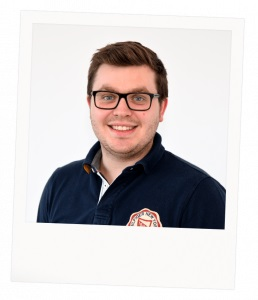
\includegraphics[width=13cm,right]{figures/Laurens.jpg} 
\end{minipage}

\vspace{1cm} % A bit of extra whitespace between the header and poster content

%----------------------------------------------------------------------------------------

\begin{multicols}{2} % This is how many columns your poster will be broken into, a portrait poster is generally split into 2 columns

%----------------------------------------------------------------------------------------
%	ABSTRACT
%----------------------------------------------------------------------------------------

\color{HoGentAccent1} % Navy color for the abstract

\begin{abstract}
De huidige generatie hogeschoolstudenten kan niet meer zonder zijn coole snufjes. Of het nu een smartphone, laptop of tablet is, elke student komt dagelijks wel met één of meer van deze apparaten in zijn rugzak naar school. Maar is dit wel altijd een meerwaarde voor de student zijn studieresultaten? Door middel van een bevraging rond te sturen voor studenten van 4 verschillende studierichtingen op zowel de Haagse Hogeschool als de Hogeschool Gent, ben ik nagegaan wat de meningen zijn van de studenten over hun smartphone- en laptopgebruik, of de tijd die ze spenderen achter een beeldscherm. Daarnaast is ook gevraagd naar de resultaten die zij behaalden in hun laatste examenperiode. Er is ook een praktijktest afgenomen waarbij studenten aan het einde van een theoretische les een aantal vragen over de net gegeven les moesten beantwoorden. In sommige klassen hadden studenten alle elektronische gadgets mogen gebruiken een hele les, in andere klassen werd opgelegd om enkel pen en papier een hele les te gebruiken. Uit deze ondervragingen blijkt dat vooral het gedrag van studenten tijdens de les een bepalende factor kan zijn voor de studieresultaten. Het aantal uur dat de student buiten de les spendeert op zijn smartphone of laptop is weinig of niet relevant. Hoe minder je als student je smartphone of laptop gebruikt tijdens de les, hoe beter je kans op slagen of een goed resultaat. Studenten met enkel pen en papier namen ook meer kennis op dan studenten die hun laptop of smartphone hadden gebruikt. Door deze resultaten is verder onderzoek bij grotere groepen studenten aangewezen.
\end{abstract}
%----------------------------------------------------------------------------------------
%	INTRODUCTION
%----------------------------------------------------------------------------------------

\color{HoGentAccent1} 
\section*{Introductie}
\color{black}
\color{black}
BYOB (Bring your own device), m-learning, e-learning, mobile learning... Dit zijn maar enkele termen die vaak gebruikt worden op middelbare of hogere scholen. Al deze termen hebben 1 doel: proberen om de student een optimale leerervaring te bieden, of deze zich nu op school voordoet of thuis. Deze nodige apparaten hiervoor kunnen namelijk voor de
meeste problemen een pasklare oplossing bieden en af en toe ook de student een klein verzetje bieden (ontspanning, games, hobby’s...). Maar is dit wel zo? Als men de cijfers van de Haagse Hogeschool erbij neemt voor de opleiding HBO-ICT, ziet men dat maar 32 procent
van alle studenten die starten aan de opleiding ook werkelijk aan hun diploma geraken binnen de 5 jaar (voor een opleiding van 4 jaar). Men kan zich dan de vraag stellen of deze apparaten in computergerichte studierichtingen wel degelijk gebruikt worden door de student als studiegereedschap. Zijn smartphones en laptops wel een motivatie om extra op te letten
of te studeren voor een schoolvak? Vormen ze niet meer een afleiding voor de student?
%----------------------------------------------------------------------------------------
%	GEOLOGY
%----------------------------------------------------------------------------------------

\color{Black} % DarkSlateGray color for the rest of the content
\color{HoGentAccent1} 
\section*{Onderzoeksvragen}
\color{black}
\begin{itemize}
	\item Heeft het gebruik van smartphones en laptops tijdens de lessen mogelijks een invloed op de slaagcijfers en (parate) kennis van de student? (Hoofdvraag)
	\item Heeft geslacht, relatiestatus of leeftijd van de student een invloed op de aantrekkingskracht die deze devices hebben op de student?
	\item Is er een verschil in omgang met devices tussen Nederlandse en Vlaamse studenten?
	\item Wat denken studenten zelf over de invloed van smartphones op hun resultaten?
	\item Is er een verschil tussen studenten uit een sociale richting en studenten uit een richting die IT-gerelateerd is?
	\item Is er een direct positief effect op de student in het klaslokaal wanneer de smartphone en laptop volledig uit beeld verdwijnen?
\end{itemize}
\begin{center}\vspace{1cm}
	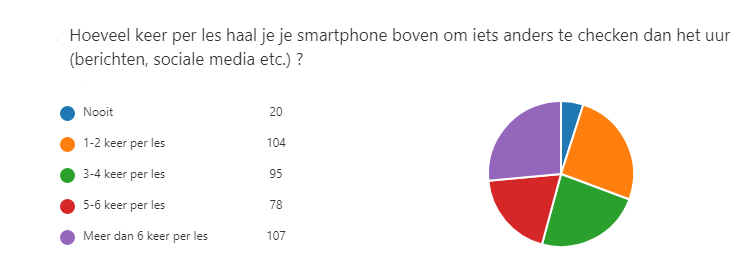
\includegraphics[width=1.0\linewidth]{smartphone-social.png}
	\captionof{figure}{\color{HoGentAccent5} Aantal keer dat studenten aangeven hun smartphone boven te halen tijdens een les volgens de enquête bij 404 studenten}
\end{center}\vspace{1cm}

\color{HoGentAccent1} 
\section*{Methodologie}
\color{black}
Dit onderzoek is opgesplitst in 2 onderzoeken. Ten eerste is gekozen om een online enquête te verspreiden onder de studenten uit de gekozen studierichtingen aan beide hogescholen. In het tweede
onderzoek is gekozen voor een test die voorgelegd werd aan de eerstejaarsstudent Toegepaste Informatica van Gent tijdens de lessen. 
\color{HoGentAccent1} 
\section*{Resultaten en Conclusie}
\color{black}
Het aantal uur dat de student buiten de les
spendeert op zijn smartphone of laptop is weinig of niet relevant. Hoe minder je je
smartphone gebruikt, hoe beter je kans op slagen of een goed resultaat. Daarnaast konden
we ook vaststellen dat vrouwen bijna een uur meer per dag spenderen op hun smartphone,
dat vrijgezellen een half uur langer per dag hun smartphone of laptop gebruiken, dat
Vlamingen meer op hun smartphone zitten maar dat bijna 9 op de 10 Nederlanders hun
laptop meebrengen naar de les, dat 6 op 10 studenten aangeeft dat smartphones en laptops
tijdens de les hen afleidt en dat studenten uit sociale richtingen 75 minuten per dag minder
achter een scherm spenderen dan IT-studenten.
\begin{center}\vspace{1cm}
	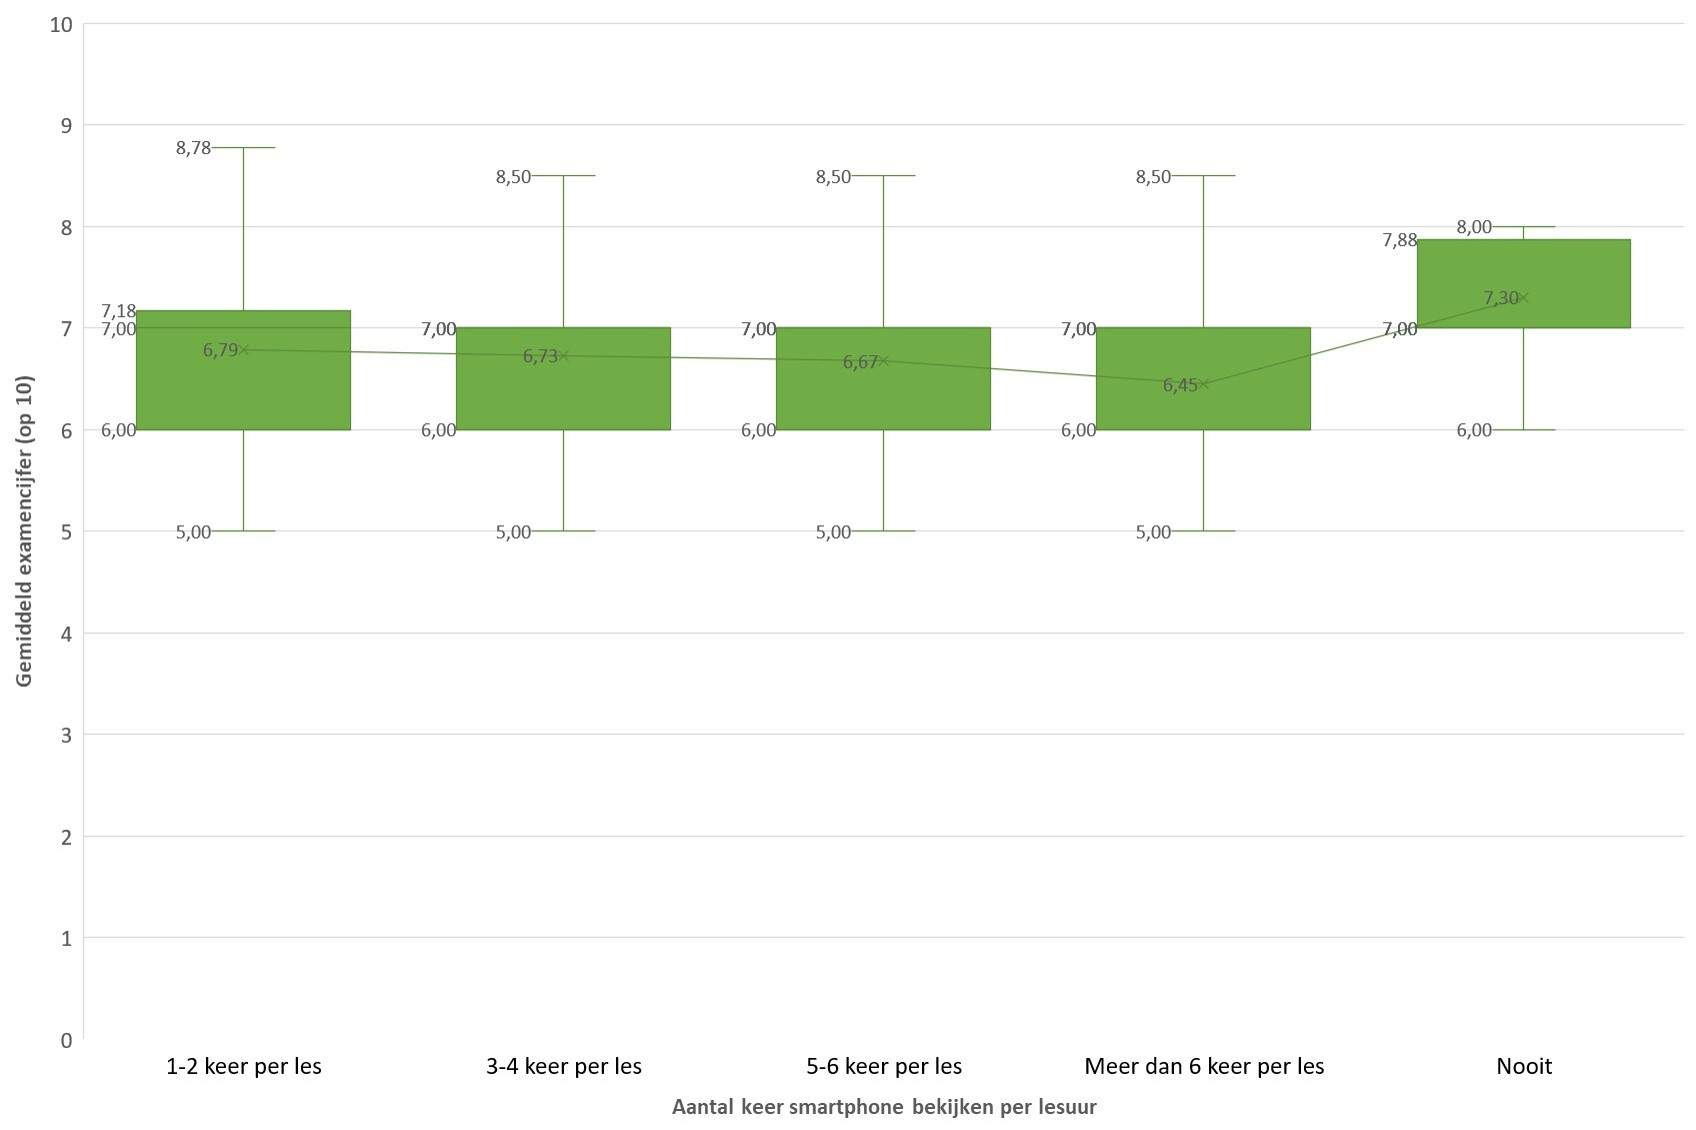
\includegraphics[scale=0.8]{Boxplot1.jpg}
	\captionof{figure}{\color{HoGentAccent5} Vergelijking tussen gemiddeld studiecijfer van student en het aantal keer dat hij of zij afgeleid is tijdens de les door smartphone}
\end{center}\vspace{1cm}
\begin{center}\vspace{1cm}
	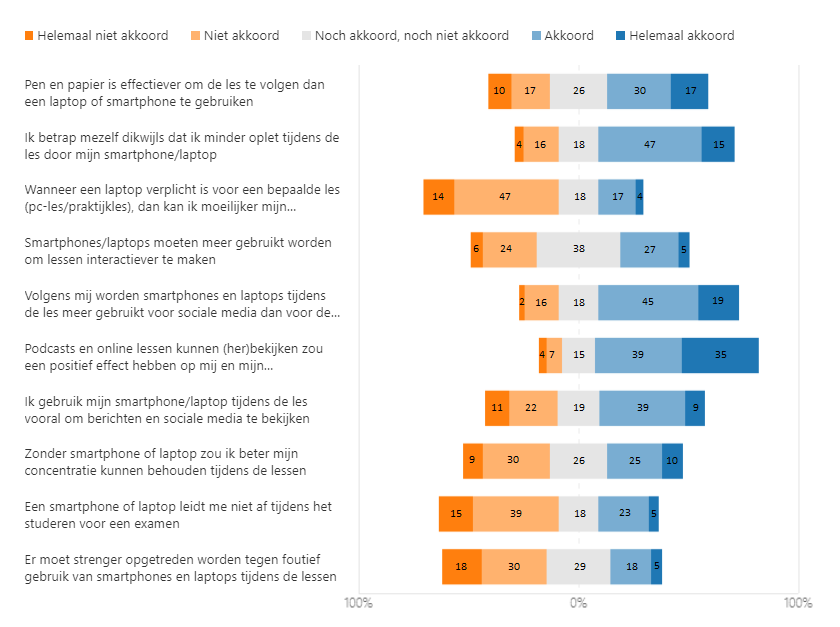
\includegraphics[scale=1.3]{stellingen.png}
	\captionof{figure}{\color{HoGentAccent5} Antwoorden van 404 studenten op 10 stellingen over hun apparaten en hun lessen}
\end{center}\vspace{1cm}

\begin{center}\vspace{1cm}
	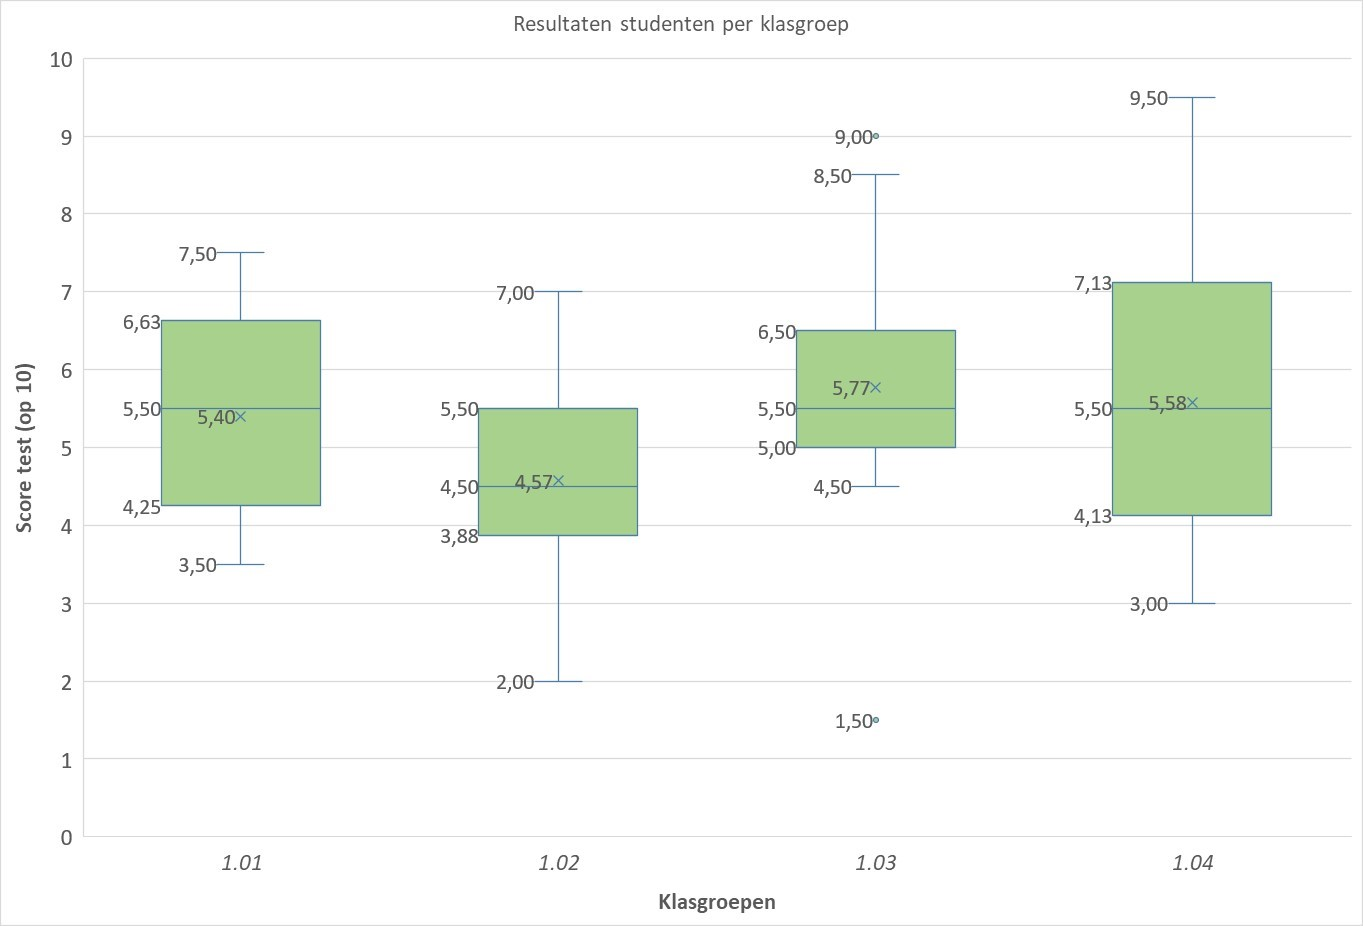
\includegraphics[scale=0.8]{Boxplot3.jpg}
	\captionof{figure}{\color{HoGentAccent5} Vergelijking van scores tussen studenten uit 4 geteste klassen Toegepaste Informatica bij het vak Probleemoplossend Denken 1 (Klassen 1.01 en 1.03 gebruikten enkel pen en papier, klassen 1.02 en 1.04 mochten alles gebruiken)}
\end{center}\vspace{1cm}

De praktijktest bracht aan het licht dat een student uit een klas waar geen smartphones of
laptops toegelaten zijn gemiddeld 5,6 procent meer kennis opnemen over de net gegeven
les dan wanneer de student in een klas zat waar smartphone en laptop toegelaten waren, en
dat, zonder te kijken naar in wat voor klas de student zit, een student die geen elektronica
gebruikt de hele les 8,3 procent meer kennis heeft over de les dan een student die ervoor
heeft gekozen om zijn smartphone of laptop te gebruiken.
%----------------------------------------------------------------------------------------
%	FORTHCOMING RESEARCH
%----------------------------------------------------------------------------------------
\color{HoGentAccent1} 
\section*{Toekomstig onderzoek}
\color{black}
Er is, ondanks de veelbelovende resultaten, nog verder onderzoek nodig om echt significante resultaten te verkrijgen over
de aangekaarte onderwerpen binnen deze bachelorproef. Er is vooral nood aan verder
onderzoek over gedrag van studenten binnen de muren van de klas. Daar wordt kennis
opgedaan die later kan beslissen over een positief of negatief resultaat voor de student zijn
examens en zijn of haar toekomst.
%----------------------------------------------------------------------------------------

\end{multicols}
\end{document}